\section{Khoa học thuật toán}
Thuở ban đầu, do khả năng lưu trữ thông tin bị giới hạn và các thủ tục lập trình dài dòng,
rắc rối nên các thuật toán được sử dụng trong các máy tính toán còn rất đơn giản. Theo
thời gian, các rào cản này dần bị phá bỏ; các máy đã được ứng dụng cho các nhiệm vụ lớn
hơn và phức tạp hơn. Việc biểu diễn các nhiệm vụ phức tạp này dưới dạng thuật toán đã bắt
đầu thách thức khả năng của con người. Chính vì vậy, ngày càng có nhiều nghiên cứu hướng
về thuật toán và lập trình.

Trong bối cảnh này, các kết quả lý thuyết của các nhà toán học mới bắt
đầu mới thể hiện tầm quan trọng của nó. Nhờ định lý về tính không toàn
vẹn của G\"odel, các nhà toán học đã bắt đầu nghiên cứu các vấn đề
liên quan đến thuật toán nảy sinh từ công nghệ cao. Từ đây, nổi lên
một nghành khoa học mới, gọi là \textit{khoa học máy tính}.

Ngày nay, khoa học máy tính cũng được coi như là như là khoa học thuật
toán. Phạm vi của ngành khoa học này rất rộng, liên quan đến cả toán
học, kỹ thuật, tâm lý học, sinh học, quản trị kinh doanh, và ngôn ngữ
học. Trong các chương tiếp theo, ta sẽ thảo luận nhiều vấn đề
khác nhau của ngành khoa học này. Với mỗi vấn đề, mục tiêu của chúng
ta bao gồm: giới thiệu các ý tưởng trung tâm, các vấn đề đang được
nghiên cứu, và một vài phương pháp đang được sử dụng để phát triển tri
thức trong lĩnh vực này.

Để có được một bức tranh tổng thể về khoa học máy tính, ta xem
xét những câu hỏi sau đây:

\begin{figure}[tb] 
\centering
    \scalebox{0.4}{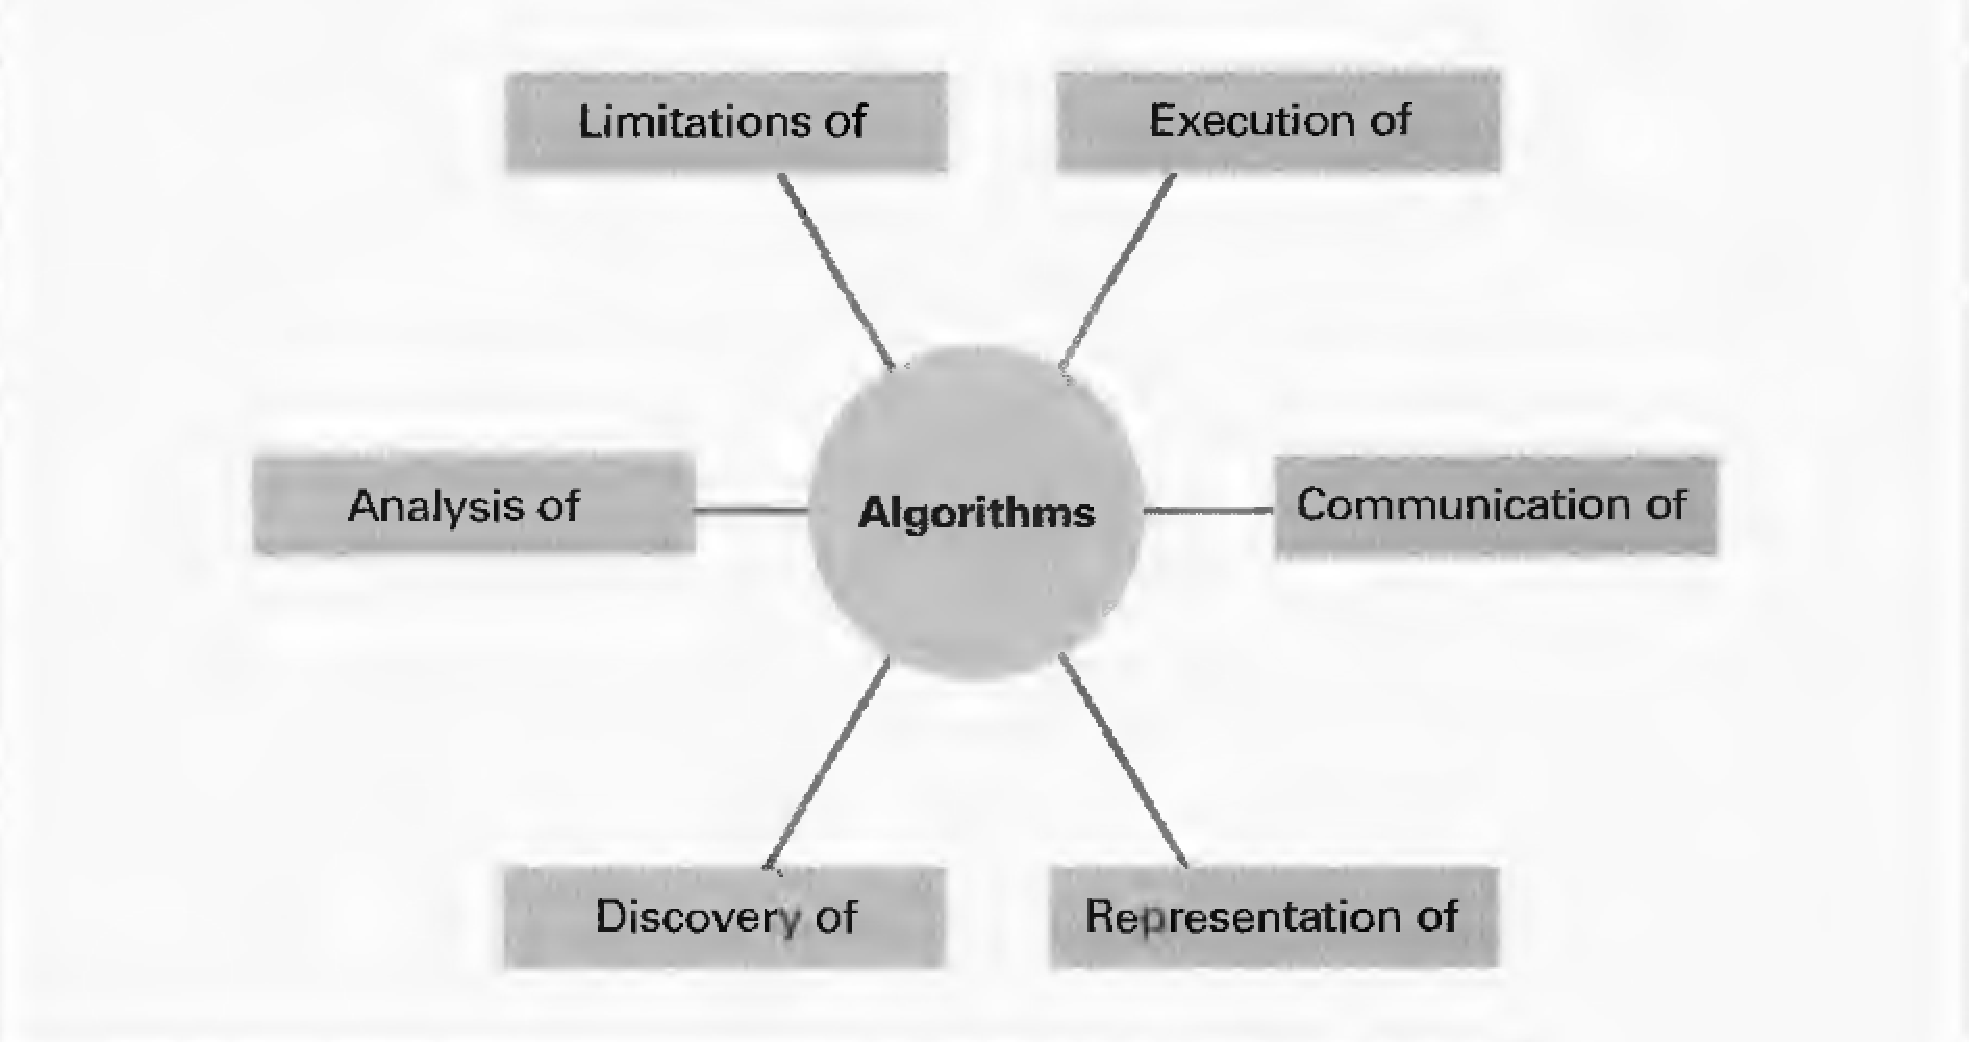
\includegraphics{ch0/fig05.pdf}}
\caption{Vai trò trung tâm của thuật toán trong khoa học máy tính}
  \label{fig:fig0.5}
\end{figure}

\begin{itemize}
\item Những bài toán nào có thể được giải bằng thuật toán?

\item Làm sao để có thể phát hiện ra thuật toán một cách dễ dàng hơn?

\item Làm sao để biểu diễn và truyền tải thuật toán một cách tốt
  hơn?

\item Làm sao để các kiến thức về thuật toán giúp ta tạo ra
  các máy tốt hơn?

\item Làm sao để có thể phân tích và so sánh các đặc trưng 
  của các thuật toán khác nhau?
\end{itemize}

Chú ý rằng các câu hỏi này đều hướng đến một chủ đề chung là nghiên
cứu thuật toán~(Hình~\ref{fig:fig0.5})




%%% Local Variables: 
%%% mode: latex
%%% TeX-master: "../tindaicuong"
%%% End: 
